\section{Conceptual Design}

\subsection{C-IDM In The Large}

\begin{figure}[h]
	\centering
	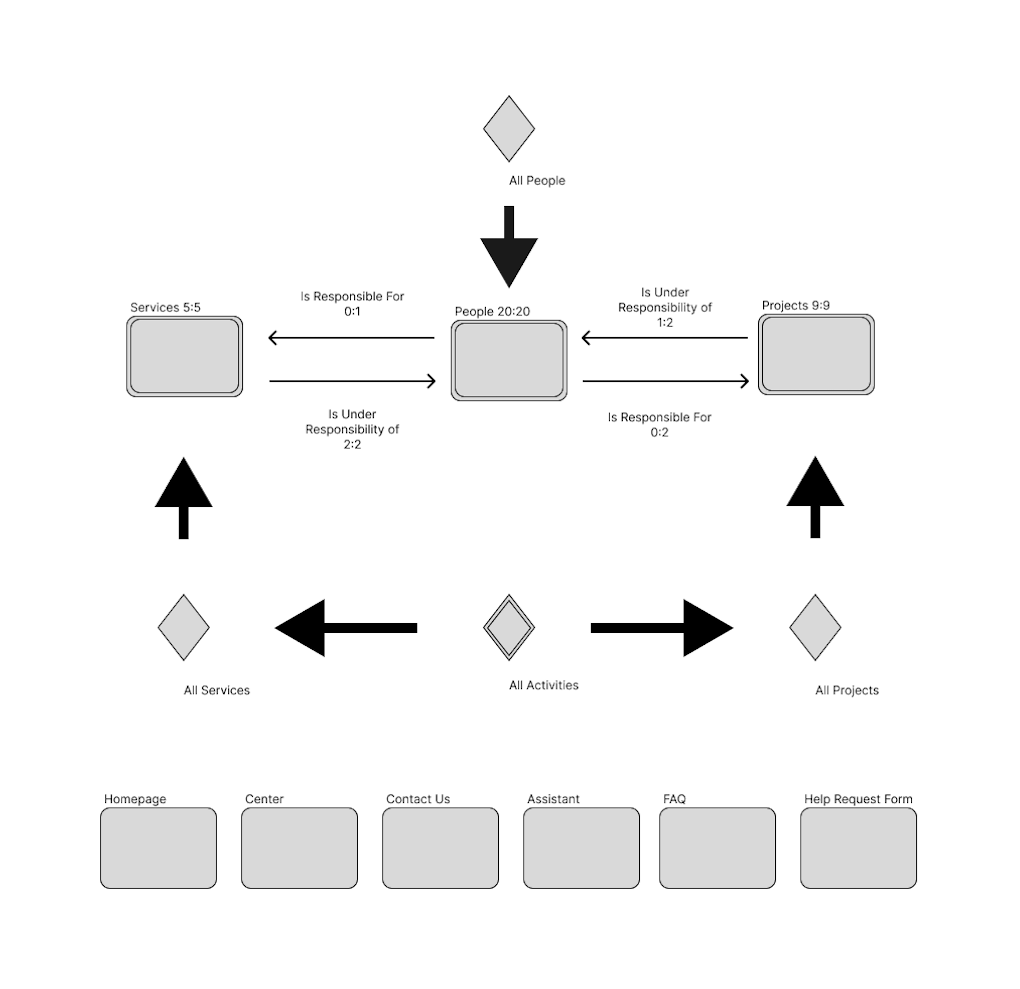
\includegraphics[width=\linewidth]{Resources/CIDM_in_large.png}
	\caption{C-IDM in the large diagram.}
	\label{fig:example}
\end{figure}


\subsection{C-IDM In The Small}
The general structure of the website was defined using the C-IDM in the large notation. 
This method ensures that particular attention is paid to the relations among topics within groups and their cardinality, 
which is defined as the expected minimum and maximum number of instances of a topic or relation.

% CIDM Image

A detailed preview of the page content was crafted using the C-IDM in the small notation, presented as Content Tables.

% Contacts
\begin{table}[htp!]
    \centering
    \begin{tabular}{ |l|l| }
        \hline
        \rowcolor{anemoneBlue}
        \multicolumn{2}{ |l| }{\color{white}{\textbf{Topic : Contacts}}}\\
        \hline
        \textbf{Title} & \texttt{Text} \color{anemoneGray}{Contacts}\\
        \hline
        \textbf{Subtitle} & \texttt{Text} \color{anemoneGray}{max 64 chars}\\
        \hline
        \textbf{Phone Number} & \texttt{Text} \color{anemoneGray}{max 64 chars}\\
        \hline
        \textbf{Email} & \texttt{Text} \color{anemoneGray}{max 64 chars}\\
        \hline
        \textbf{Address} & \texttt{Text} \color{anemoneGray}{max 128 chars}\\
        \hline
        \textbf{Map} & \texttt{Interactive Map}\\
        \hline
    \end{tabular}
\end{table}

% Assistant
\begin{table}[htp!]
    \centering
    \begin{tabular}{ |l|l| }
        \hline
        \rowcolor{anemoneBlue}
        \multicolumn{2}{ |l| }{\color{white}{\textbf{Kinf of Topic : Chatbot}}}\\
        \hline
        \textbf{Chatbot Name} & \texttt{Text (max 64 chars)}\\
        \hline
        \textbf{Tag Line} & \texttt{Text (max 64 chars)}\\
        \hline
        \textbf{Chat Conversation} & \texttt{Scrollable Text Box} \\
        \hline
        \textbf{User Input} & \texttt{Text Input Box (max 200 chars)}\\
        \hline
    \end{tabular}
\end{table}

% Person
\begin{table}[htp!]
    \centering
    \begin{tabular}{ |l|l| }
        \hline
        \rowcolor{anemoneBlue}
        \multicolumn{2}{ |l| }{\color{white}{\textbf{Kinf of Topic : Person}}}\\
        \hline
        \textbf{Name} & \texttt{Text (max 64 chars)}\\
        \hline
        \textbf{Picture of Person} & \texttt{Image} \\
        \hline
        \textbf{CV} & \texttt{Text (max 200 words)}\\
        \hline
        \textbf{Role} & \texttt{Text (max 64 chars)}\\
        \hline
        \textbf{Activities} & \texttt{List of [Links(Activity Name)]}\\
        \hline
    \end{tabular}
\end{table}

% Project
\begin{table}[htp!]
    \centering
    \begin{tabular}{ |l|l| }
        \hline
        \rowcolor{anemoneBlue}
        \multicolumn{2}{ |l| }{\color{white}{\textbf{Kinf of Topic : Project}}}\\
        \hline
        \textbf{Project Name} & \texttt{Text (max 64 chars)}\\
        \hline
        \textbf{Picture of Project} & \texttt{Image} \\
        \hline
        \textbf{Short Description} & \texttt{Text (max 200 words)}\\
        \hline
    \end{tabular}
\end{table}

% Service
\begin{table}[htp!]
    \centering
    \begin{tabular}{ |l|l| }
        \hline
        \rowcolor{anemoneBlue}
        \multicolumn{2}{ |l| }{\color{white}{\textbf{Kinf of Topic : Service}}}\\
        \hline
        \textbf{Service Name} & \texttt{Text (max 64 chars)}\\
        \hline
        \textbf{Tag Line} & \texttt{Text (max 64 chars)}\\
        \hline
        \textbf{Picture of Service} & \texttt{Image} \\
        \hline
        \textbf{Description and Benefits} & \texttt{Text (max 200 words)}\\
        \hline
        \textbf{Availability} & \texttt{Text (max 200 words)}\\
        \hline
        \textbf{Testimonial} & \texttt{Text (max 100 words)}\\
        \hline
    \end{tabular}
\end{table}

% Centre
\begin{table}[htp!]
    \centering
    \begin{tabular}{ |l|l| }
        \hline
        \rowcolor{anemoneBlue}
        \multicolumn{2}{ |l| }{\color{white}{\textbf{Topic : Centre}}}\\
        \hline
        \textbf{Title} & \texttt{Text (max 64 chars)}\\
        \hline
        \textbf{History and Mission} & \texttt{Text (max 100 words)}\\
        \hline
        \textbf{Opening Hours} & \texttt{Text (max 100 words)}\\
        \hline
        \textbf{Address} & \texttt{Text (max 64 chars)}\\
        \hline
        \textbf{Map} & \texttt{Interactive Map}\\
        \hline
    \end{tabular}
\end{table}



% FAQ
\begin{table}[htp!]
    \centering
    \begin{tabular}{ |l|l| }
        \hline
        \rowcolor{anemoneBlue}
        \multicolumn{2}{ |l| }{\color{white}{\textbf{Topic : FAQ}}}\\
        \hline
        \textbf{Title} & \texttt{Text} \color{anemoneGray}{max 32 chars}\\
        \hline
        \textbf{Description} & \texttt{Text} \color{anemoneGray}{max 576 chars}\\
        \hline
    \end{tabular}
\end{table}

% All People
\begin{table}[htp!]
    \centering
    \begin{tabular}{ |l|l| }
        \hline
        \rowcolor{anemoneBlue}
        \multicolumn{2}{ |l| }{\color{white}{\textbf{Group : People}}}\\
        \hline
        \textbf{Title} & \texttt{Text (max 64 chars)}\\
        \hline
        \textbf{Tag Line} & \texttt{Text (max 64 chars)}\\
        \hline
        \textbf{Persons} & \texttt{List of [Name, Profile Image, Role]}\\
        \hline
    \end{tabular}
\end{table}

% All Projects
\begin{table}[htp!]
    \centering
    \begin{tabular}{ |l|l| }
        \hline
        \rowcolor{anemoneBlue}
        \multicolumn{2}{ |l| }{\color{white}{\textbf{Group : Projects}}}\\
        \hline
        \textbf{Title} & \texttt{Text (max 64 chars)}\\
        \hline
        \textbf{Tag Line} & \texttt{Text (max 64 chars)}\\
        \hline
        \textbf{Projects} & \texttt{List of [Name, Project Image, Description]}\\
        \hline
    \end{tabular}
\end{table}

% All Services
\begin{table}[htp!]
    \centering
    \begin{tabular}{ |l|l| }
        \hline
        \rowcolor{anemoneBlue}
        \multicolumn{2}{ |l| }{\color{white}{\textbf{Group : Services}}}\\
        \hline
        \textbf{Title} & \texttt{Text (max 64 chars)}\\
        \hline
        \textbf{Tag Line} & \texttt{Text (max 64 chars)}\\
        \hline
        \textbf{Services} & \texttt{List of [Name, Service Image, Description]}\\
        \hline
    \end{tabular}
\end{table}







\subsection{Abstract Pages}

% Homepage
\begin{table}[htp!]
    \centering
    \begin{tabular}{ |l|l|l| }
        \hline
        \rowcolor{anemoneBlue}
        \multicolumn{3}{ |l| }{\color{white}{\textbf{Topic : Homepage}}}\\
        \hline
        \texttt{ Landmarks } &  \textbf{NavBar} & \texttt{Links to Assistant, Center, Projects, Services, People}\\
        \hline
        \texttt{  }  & \textbf{Picture} & \texttt{Image} \\
        \hline
         \texttt{  } &\textbf{Center Name} & \texttt{Text (max 64 chars)} \\
        \hline
        \texttt{  } &\textbf{Tag Line} & \texttt{Text (max 64 chars)} \\
        \hline
        \texttt{  }  & \textbf{Description} & \texttt{Text (max 100 words)}\\
        \hline
        \texttt{ Transition Link }  & \textbf{Help Button} & \texttt{Link to Request Help Page}\\
        \hline
        \texttt{ Landmarks } &  \textbf{Footer} & \texttt{Links to Contacts, Instagram, X (Twitter), FAQ}\\
        \hline
    \end{tabular}
\end{table}

% Contacts
\begin{table}[htp!]
    \centering
    \begin{tabular}{ |l|l|l| }
        \hline
        \rowcolor{anemoneBlue}
        \multicolumn{3}{ |l| }{\color{white}{\textbf{Topic : Contacts}}}\\
        \hline
        \texttt{ Landmarks } &  \textbf{NavBar} & \texttt{Links to Assistant, Center, Projects, Services, People}\\
        \hline
        \texttt{  } & \textbf{Title} & \texttt{Text} \color{anemoneGray}{Contacts}\\
        \hline
        \texttt{  } & \textbf{Subtitle} & \texttt{Text} \color{anemoneGray}{max 64 chars}\\
        \hline
        \texttt{  } & \textbf{Phone Number} & \texttt{Text} \color{anemoneGray}{max 64 chars}\\
        \hline
        \texttt{  } & \textbf{Email} & \texttt{Text} \color{anemoneGray}{max 64 chars}\\
        \hline
        \texttt{  } & \textbf{Address} & \texttt{Text} \color{anemoneGray}{max 128 chars}\\
        \hline
        \texttt{  } & \textbf{Map} & \texttt{Interactive Map}\\
        \hline
        \texttt{ Landmarks } &  \textbf{Footer} & \texttt{Links to Contacts, Instagram, X (Twitter), FAQ}\\
        \hline
    \end{tabular}
\end{table}

% Assistant
\begin{table}[htp!]
    \centering
    \begin{tabular}{ |l|l|l| }
        \hline
        \rowcolor{anemoneBlue}
        \multicolumn{3}{ |l| }{\color{white}{\textbf{Topic : Chatbot}}}\\
        \hline
        \texttt{ Landmarks } &  \textbf{NavBar} & \texttt{Links to Assistant, Center, Projects, Services, People}\\
        \hline
        \texttt{  } & \textbf{Chatbot Name} & \texttt{Text (max 64 chars)}\\
        \hline
        \texttt{  } & \textbf{Tag Line} & \texttt{Text (max 64 chars)}\\
        \hline
        \texttt{  } & \textbf{Chat Conversation} & \texttt{Scrollable Text Box} \\
        \hline
        \texttt{  } & \textbf{User Input} & \texttt{Text Input Box (max 200 chars)}\\
        \hline
        \texttt{ Landmarks } &  \textbf{Footer} & \texttt{Links to Contacts, Instagram, X (Twitter), FAQ}\\
        \hline
    \end{tabular}
\end{table}

% Person
\begin{table}[htp!]
    \centering
    \begin{tabular}{ |l|l|l| }
        \hline
        \rowcolor{anemoneBlue}
        \multicolumn{3}{ |l| }{\color{white}{\textbf{Kind of Topic : Person}}}\\
        \hline
        \texttt{ Landmarks } &  \textbf{NavBar} & \texttt{Links to Assistant, Center, Projects, Services, People}\\
        \hline
         \texttt{  } &\textbf{Name} & \texttt{Text (max 64 chars)} \\
        \hline
        \texttt{  }  & \textbf{Picture of Person} & \texttt{Image} \\
        \hline
        \texttt{  }  & \textbf{CV} & \texttt{Text (max 200 words)}\\
        \hline
        \texttt{  }  & \textbf{Role} & \texttt{Text (max 64 chars)}\\
        \hline
         \texttt{ Transition Links }  & \textbf{Activities} & \texttt{List of [Links(Activity Name)]}\\
        \hline
        \texttt{ Landmarks } &  \textbf{Footer} & \texttt{Links to Contacts, Instagram, X (Twitter), FAQ}\\
        \hline
    \end{tabular}
\end{table}



% Project
\begin{table}[htp!]
    \centering
    \begin{tabular}{ |l|l|l| }
        \hline
        \rowcolor{anemoneBlue}
        \multicolumn{3}{ |l| }{\color{white}{\textbf{Kinf of Topic : Project}}}\\
        \hline
        \texttt{ Landmarks } &  \textbf{NavBar} & \texttt{Links to Assistant, Center, Projects, Services, People}\\
        \hline
        \texttt{  } & \textbf{Project Name} & \texttt{Text (max 64 chars)}\\
        \hline
        \texttt{  } & \textbf{Tag Line} & \texttt{Text (max 64 chars)}\\
        \hline
        \texttt{  } & \textbf{Picture of Project} & \texttt{Image} \\
        \hline
        \texttt{  } & \textbf{Short Description} & \texttt{Text (max 200 words)}\\
        \hline
        \texttt{ Landmarks } &  \textbf{Footer} & \texttt{Links to Contacts, Instagram, X (Twitter), FAQ}\\
        \hline
    \end{tabular}
\end{table}

% Service
\begin{table}[htp!]
    \centering
    \begin{tabular}{ |l|l|l| }
        \hline
        \rowcolor{anemoneBlue}
        \multicolumn{3}{ |l| }{\color{white}{\textbf{Kinf of Topic : Service}}}\\
        \hline
        \texttt{ Landmarks } &  \textbf{NavBar} & \texttt{Links to Assistant, Center, Projects, Services, People}\\
        \hline
        \texttt{  } & \textbf{Service Name} & \texttt{Text (max 64 chars)}\\
        \hline
        \texttt{  } & \textbf{Tag Line} & \texttt{Text (max 64 chars)}\\
        \hline
        \texttt{  } & \textbf{Picture of Service} & \texttt{Image} \\
        \hline
        \texttt{  } & \textbf{Description and Benefits} & \texttt{Text (max 200 words)}\\
        \hline
        \texttt{  } & \textbf{Availability} & \texttt{Text (max 200 words)}\\
        \hline
        \texttt{  } & \textbf{Testimonial} & \texttt{Text (max 100 words)}\\
        \hline
        \texttt{ Landmarks } &  \textbf{Footer} & \texttt{Links to Contacts, Instagram, X (Twitter), FAQ}\\
        \hline
    \end{tabular}
\end{table}

% Centre
\begin{table}[htp!]
    \centering
    \begin{tabular}{ |l|l|l| }
        \hline
        \rowcolor{anemoneBlue}
        \multicolumn{3}{ |l| }{\color{white}{\textbf{Topic : Centre}}}\\
        \hline
        \texttt{ Landmarks } &  \textbf{NavBar} & \texttt{Links to Assistant, Center, Projects, Services, People}\\
        \hline
        \texttt{  } & \textbf{Title} & \texttt{Text (max 64 chars)}\\
        \hline
        \texttt{  } & \textbf{Tag Line} & \texttt{Text (max 64 chars)}\\
        \hline
        \texttt{  } & \textbf{History and Mission} & \texttt{Text (max 100 words)}\\
        \hline
        \texttt{  } & \textbf{Opening Hours} & \texttt{Text (max 100 words)}\\
        \hline
        \texttt{  } & \textbf{Address} & \texttt{Text (max 64 chars)}\\
        \hline
        \texttt{  } & \textbf{Map} & \texttt{Interactive Map}\\
        \hline
        \texttt{ Landmarks } &  \textbf{Footer} & \texttt{Links to Contacts, Instagram, X (Twitter), FAQ}\\
        \hline
    \end{tabular}
\end{table}



% FAQ
\begin{table}[htp!]
    \centering
    \begin{tabular}{ |l|l|l|}
        \hline
        \rowcolor{anemoneBlue}
        \multicolumn{3}{ |l| }{\color{white}{\textbf{Topic : FAQ}}}\\
        \hline
        \texttt{ Landmarks } &  \textbf{NavBar} & \texttt{Links to Assistant, Center, Projects, Services, People}\\
        \hline
        \texttt{  } & \textbf{Title} & \texttt{Text (max 64 chars)}\\
        \hline
        \texttt{  } & \textbf{Description} & \texttt{ Text (max 100 words)}\\
        \hline
        \texttt{ Landmarks } &  \textbf{Footer} & \texttt{Links to Contacts, Instagram, X (Twitter), FAQ}\\
        \hline
    \end{tabular}
\end{table}

% All People
\begin{table}[htp!]
    \centering
    \begin{tabular}{ |l|l|l| }
        \hline
        \rowcolor{anemoneBlue}
        \multicolumn{3}{ |l| }{\color{white}{\textbf{Group : People}}}\\
        \hline
        \texttt{ Landmarks } &  \textbf{NavBar} & \texttt{Links to Assistant, Center, Projects, Services, People}\\
        \hline
        \texttt{  } & \textbf{Title} & \texttt{Text (max 64 chars)}\\
        \hline
        \texttt{  } & \textbf{Tag Line} & \texttt{Text (max 64 chars)}\\
        \hline
        \texttt{ Group Links } & \textbf{Persons} & \texttt{List of [Name, Profile Image, Role]}\\
        \hline
        \texttt{ Landmarks } &  \textbf{Footer} & \texttt{Links to Contacts, Instagram, X (Twitter), FAQ}\\
        \hline
    \end{tabular}
\end{table}

% All Projects
\begin{table}[htp!]
    \centering
    \begin{tabular}{ |l|l|l| }
        \hline
        \rowcolor{anemoneBlue}
        \multicolumn{3}{ |l| }{\color{white}{\textbf{Group : Projects}}}\\
        \hline
        \texttt{ Landmarks } &  \textbf{NavBar} & \texttt{Links to Assistant, Center, Projects, Services, People}\\
        \hline
        \texttt{  } & \textbf{Title} & \texttt{Text (max 64 chars)}\\
        \hline
        \texttt{  } & \textbf{Tag Line} & \texttt{Text (max 64 chars)}\\
        \hline
        \texttt{ Group Links } & \textbf{Projects} & \texttt{List of [Name, Project Image, Description]}\\
        \hline
        \texttt{ Landmarks } &  \textbf{Footer} & \texttt{Links to Contacts, Instagram, X (Twitter), FAQ}\\
        \hline
    \end{tabular}
\end{table}

% All Services
\begin{table}[htp!]
    \centering
    \begin{tabular}{ |l|l|l| }
        \hline
        \rowcolor{anemoneBlue}
        \multicolumn{3}{ |l| }{\color{white}{\textbf{Group : Services}}}\\
        \hline
        \texttt{ Landmarks } &  \textbf{NavBar} & \texttt{Links to Assistant, Center, Projects, Services, People}\\
        \hline
        \texttt{  } & \textbf{Title} & \texttt{Text (max 64 chars)}\\
        \hline
        \texttt{  } & \textbf{Tag Line} & \texttt{Text (max 64 chars)}\\
        \hline
        \texttt{ Group Links } &  \textbf{Services} & \texttt{List of [Name, Service Image, Description]}\\
        \hline
        \texttt{ Landmarks } &  \textbf{Footer} & \texttt{Links to Contacts, Instagram, X (Twitter), FAQ}\\
        \hline
    \end{tabular}
\end{table}

\subsection{Mapping}
The content tables in the preceding section have the same name as the pages they represent. 
The following section presents the manner in which they are connected.

\subsection{PIDM Diagram}
The P-IDM notation was used to define the navigation capabilities of the website. 
This resulted in a tree-like structure with the homepage as the root, from which every page is eventually reachable.

% PIDM Image